%!TEX root = FreeRtos ARM uController.tex
\subsection{Komplexität durch Nebenläufigkeit - Debugging von Echtzeitsystemen}
\label{sec:Debugging von Echtzeitsystemen}
Under Construction :D

Durch die Einsatz eines Echtzeitbetriebssystems erhält der Entwickler einige Vorteile die bereits in Abschnitt \ref{sec:Echtzeitsysteme} beschrieben wurden. Im Gegenzug entstehen aber durch die Nebenläufigkeit neue mögliche Fehlerquellen. Viele dieser Fehler, lassen sich nicht einfach analysieren und enden beispielsweise im HardFault Handler. Welche Hilfsmittel einem Entwickler speziell bei FreeRTOS (auf STM32F4) zur Verfügung stehen und welche Fehler häufig auftreten ist der Inhalt dieses Abschnitts. Die Arten von Fehler die in einem Echtzeitsystem häufig auftreten lassen sich grob in zwei Kategorien aufteilen:
\begin{itemize}
	\item Stackoverflow
	\item Synchronisatiosfehler
\end{itemize}
Bekannte Probleme detailliert erklärt in \cite{9783827373427}
\begin{itemize}
	\item dining philosopherproblem
	\item reader and writers problem
	\item producer consumer problem (starvation)
\end{itemize}
     

\begin{figure}[ht!]
	\centering
		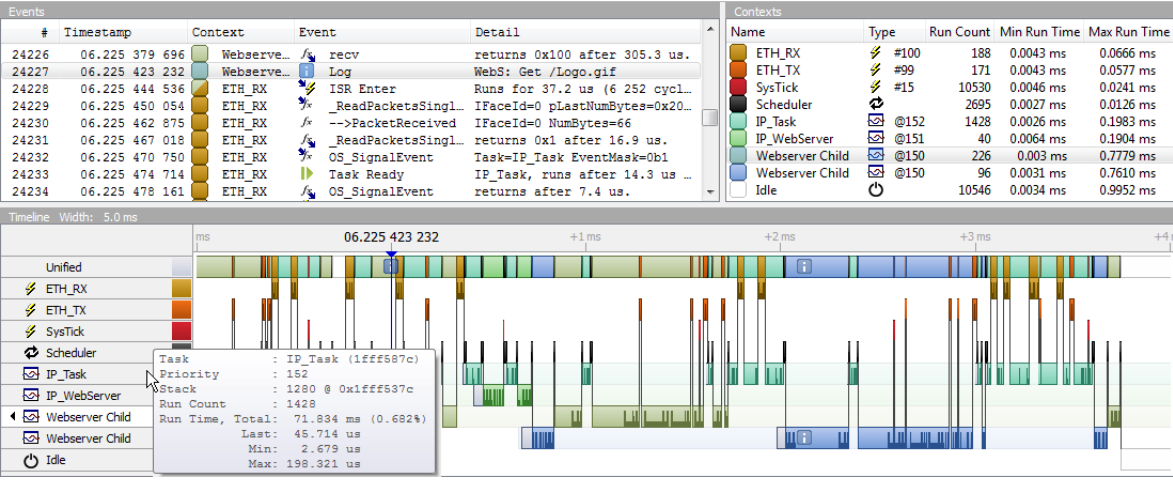
\includegraphics[width=0.5\textwidth]{Pictures/Segger/systemview.png}
	\caption{Segger Systemview - Not referenced yet}
	\label{fig:Systemview}
\end{figure}
\begin{figure}[ht!]
	\centering
		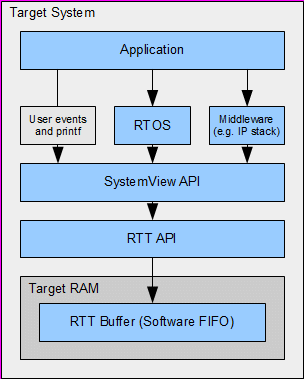
\includegraphics[width=0.3\textwidth]{Pictures/Segger/SystemViewTarget.png}
	\caption{Segger Systemview Target - Not referenced yet}
	\label{fig:SystemviewTarget}
\end{figure}
\begin{figure}[ht!]
	\centering
		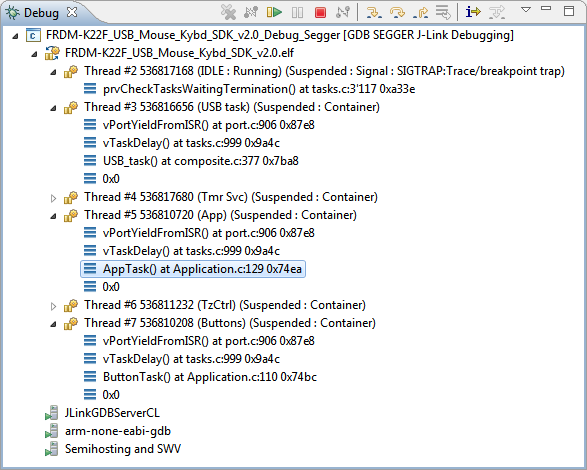
\includegraphics[width=0.5\textwidth]{Pictures/Segger/freertosThreadAwareness}
	\caption{Segger Thread Awareness- Not referenced yet}
	\label{fig:ThreadAware}
\end{figure}